\pagebreak

\subsection{Baseline Testing}
\label{sec:results-exploratory-config}

We performed initial exploratory testing with the \ac{RADOS} backend using the \ac{RDMA} and \ac{TCP} network protocols, as well as Omni-Path and InfiniBand networking, in order to determine the system and cluster configurations which were used for extended testing. Due to the time frame in which these benchmarks were run, we used Ceph v19.2.0 (Reef) instead of v20.2.0 (Tentacle) for these performance tests; the system configuration is shown in~\cref{tbl:benchmark-conditions-explore}. It is possible that newer Ceph versions may have impacted the performance results; however, the \acs{RDMA} code within Ceph has not undergone significant changes between these versions\footnote{\url{https://github.com/ceph/ceph/commits/main/src/msg/async/rdma}. Accessed 26.02.2026.}, and these results were gathered with the primary purpose of narrowing down our selection for the extended testing phase, rather than direct evaluation.

\begin{table}[H]
\centering
\begin{tabular}{|ll|}
\hline
Ceph Version       & v19.2.0 \\
Ceph Nodes         & 8 \\
Client Nodes       & 2--8 \\
Colocation         & Separate server/client nodes \\
Client Tasks       & 2--512, $1\leq t \leq 128$ per node \\
Monitors           & 1 (on node 1) \\
Managers           & 1 (on node 1) \\
\acp{OSD}          & 128 (on nodes 1--8, 16 \acp{OSD}/node) \\
\ac{OSD} size      & 12 GiB/\ac{OSD} \\
Pool Type          & Replica 3 \\
\hline
\end{tabular}
\caption[Benchmarking Conditions for Exploratory Testing]{Cluster configuration for exploratory testing.}
\label{tbl:benchmark-conditions-explore}
\end{table}

\subsubsection{Omni-Path Issues}
\label{sec:results-opa-issues}

During our initial validation runs, we were unable to collect Ceph results reliably from the nodes equipped with Omni-Path networking. The test suite was not able to complete successfully without node failures during the testing phase, which occurred on both client and cluster nodes. As a result, we have only been able to gather a limited amount of Omni-Path performance data.

\begin{figure}[H]
    \centering
    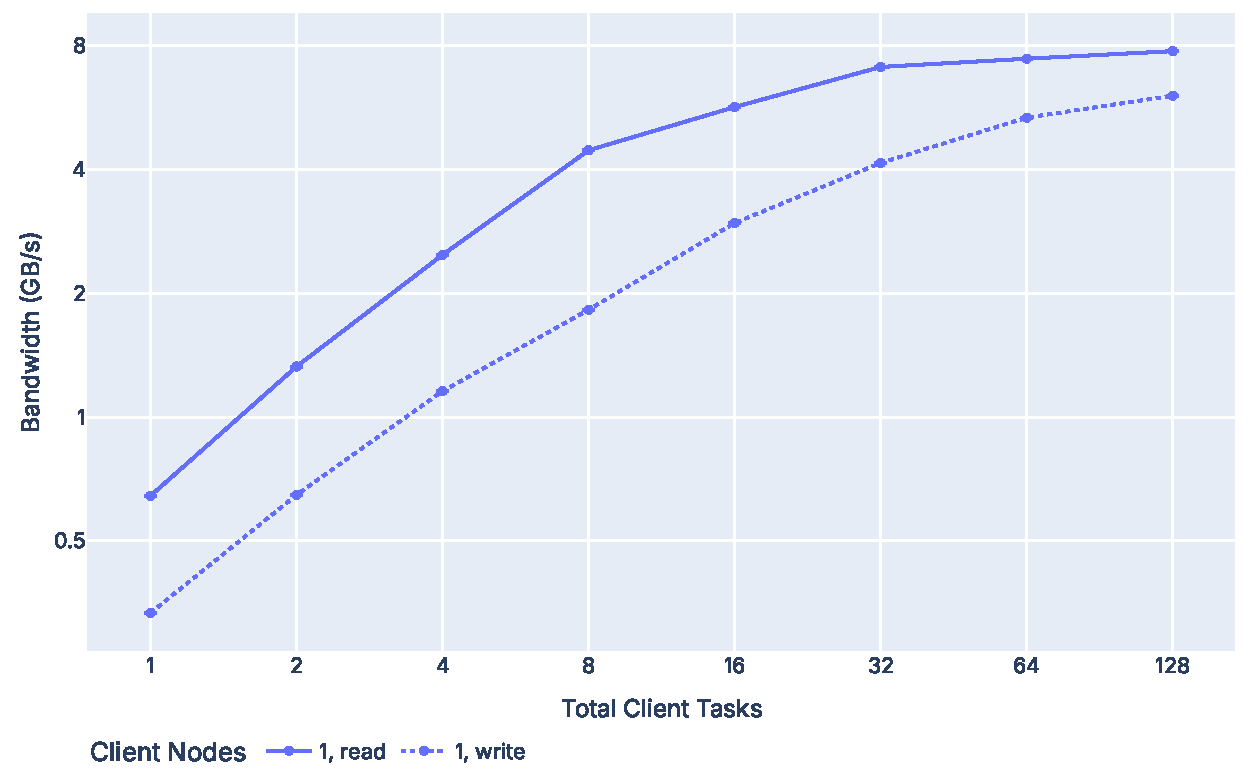
\includegraphics[width=0.9\linewidth]{assets/perf_results/omnipath_seq_64m.pdf}
    \caption[RADOS 64MiB Omni-Path Performance]{Performance results for 64MiB \acs{RADOS} read/write operations over the Omni-Path network transport.}
    \label{fig:omnipath-seq-64m}
\end{figure}

\Cref{fig:omnipath-seq-64m} shows good scaling performance results. Based on the network performance tests performed in~\cref{sec:results-network-bandwidth-opa}, peak performance is likely being limited by network performance, rather than Ceph itself.

\begin{figure}[H]
    \centering
    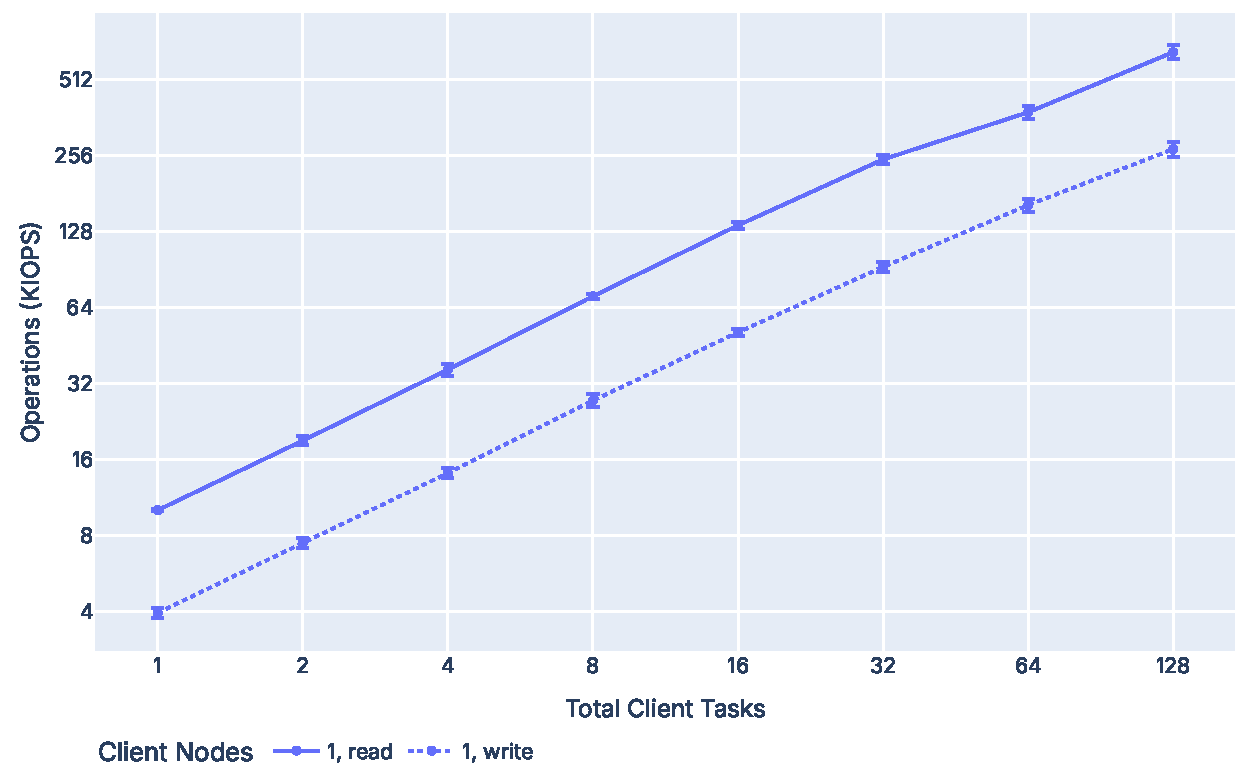
\includegraphics[width=0.9\linewidth]{assets/perf_results/omnipath_4k_iops.pdf}
    \caption[RADOS 4KiB Omni-Path Performance]{Performance results for 4KiB \acs{RADOS} read/write operations on 2MiB objects over the Omni-Path network transport.}
    \label{fig:omnipath-seq-4k}
\end{figure}

\Cref{fig:omnipath-seq-4k} demonstrates close to linear scaling for 4KiB read and write operations, suggesting a performance bottleneck primarily on the client side.

The partial performance results suggest that Omni-Path could be a suitable network platform for Ceph. However, the node failures effectively made Ceph unusable on the Omni-Path platform. Therefore, we investigated the source of the issue further.

\subsubsection{Root Cause Analysis for Omni-Path Kernel Panics}
\label{sec:opa-bad-root-cause-analysis}

Following discussions with system administrators, it was confirmed that the affected nodes could only be reached through their out-of-band management interfaces. This ruled out possible firewall restrictions or rate limits, which were not in place for such traffic. These causes were therefore excluded from consideration.

To rule out hardware defects, additional experiments were performed on the nodes within the same cluster partition (medium96s). These nodes exhibited identical failures to those initially observed. The standard96 partition was also tested: this partition contains a different hardware configuration, as shown in~\cref{tbl:standard96-system}.

\begin{table}[H]
\centering
\begin{tabular}{|ll|}
\hline
\textbf{Component} & \textbf{Specification} \\
\hline
CPU        & 2$\times$ Intel Xeon Platinum 9242 (48C/96T per CPU) \\
RAM        & 384 GB \\
Networking & 100 Gbps Omni-Path (Intel HFI100) \\
\hline
\end{tabular}
\caption[Omni-Path Failure Test Hardware]{The hardware configuration of the second cluster partition \texttt{standard96}, used to reproduce the Omni-Path kernel panic issue and exclude issues specific to the \texttt{medium96s} partition.}
\label{tbl:standard96-system}
\end{table}

Node failures persisted under this configuration. Based on this information, the causes were narrowed down to a possible issue with the software stack or the Omni-Path networking itself, rather than other hardware-specific issues.

After exclusion of these factors, the hypothesis was that the kernel, or possibly some other element in the software stack, was failing, leading to
system instability. 
In order to test this hypothesis, kernel logs were collected during benchmark execution. 
This task was made somewhat more complex due to the cluster nodes' boot method; nodes boot from the network and copy the image contents into a volatile file system (tmpfs) stored in-memory\footref{appendix:tmpfs-in-memory}. 
Any collected logs would therefore be lost on node failure or reboot, and no elevated privileges were available to change this behaviour\footref{appendix:dmesg-unprivileged}. 
As a workaround to this limitation, two methods were employed in an attempt to stream kernel logs gathered via the \texttt{dmesg -w} command prior to system failure, namely writing kernel logs to a local disk mounted at \texttt{/local}, and streaming kernel output via the network to a separate node not part of the Ceph cluster.

As a result of the kernel panic causing system halts, some failures did not write usable logs, either to the disk or via the network. 
Ultimately, after several attempts, a single useful log was recovered from a failed system via the network, via the node's secondary Ethernet network interface. The relevant sections of the collected logs are shown in \Cref{lst:opa-crash}.

\pagebreak
\lstinputlisting[
    caption={
        [Omni-Path Related Kernel Panic]
        Omni-Path related kernel panic. The source of the kernel panic is an invalid pointer access in the \texttt{hfi1\_ipoib\_send\_dma\_common} function, triggered by \ac{TCP} network activity from the
        Ceph traffic.
    },
    label={lst:opa-crash},
    frame=single,
    breaklines=true
]{assets/network/opa_crash.txt}

Searching for this specific cause, \texttt{hfi1\_ipoib\_send\_dma\_common},
leads to a report of a vulnerability (CVE-2024-26766). At the time, however, the \ac{RHEL} 8
kernel on which Rocky Linux 8 is based was reported as not affected by the
vulnerability.

Based on the bug description, we attempted to reproduce the issue in order to narrow down this issue as a possible cause of the node failures by constructing a proof-of-concept to generate an unaligned message with the correct number of \ac{SDMA} descriptors. An upstream \ac{RHEL} 8 installation was used, installed on the Omni-Path performance testing system previously detailed in~\cref{tbl:validation-system} to verify the bug stems from the upstream kernel.

\pagebreak
\lstinputlisting[
    caption={
        [Kernel Panic with Reproducer \acs{PoC}]
        Kernel panic triggered by the reproducer proof-of-concept code.
    },
    label={lst:opa-crash-poc-dmesg},
    frame=single,
    breaklines=true
]{assets/network/bug/crash-ryzen.txt}

Running the reproducer code reliably triggered the kernel panic as shown in~\cref{lst:opa-crash-poc-dmesg}; however, the exact location of the kernel panic was different to that of the Ceph-traffic-induced panic. Running this code on the same system with \ac{RHEL} 9 installed did not result in a kernel panic.

As the issue could successfully be reproduced, and because the issue represents a moderate security vulnerability of the \ac{RHEL} kernel itself rather than issues specific to our testing, the \ac{PoC} and associated report details were submitted to Red Hat privately for resolution. The vulnerability status was acknowledged and updated by Red Hat, and a security patch was released by Red Hat on 02.02.2026\footnote{\url{https://access.redhat.com/errata/RHSA-2026:1662}. Accessed 02.02.2026.}. As of 15.02.2026, the fixed kernel version (4.18.0-553.100.1.el8\_10) is provided by Rocky Linux\footnote{Kernel updates were checked on a Rocky Linux 8.10 installation.}. However, due to time constraints, it was not possible to perform additional Ceph performance testing on the Omni-Path network transport. Additionally, at the time of writing, the cluster kernel was not yet updated to this patched version. However, a manually patched \texttt{hfi1} kernel module applying the fixes for the vulnerability was successfully tested on a single node with root access provided by the cluster administrators.

\subsubsection{Transport Comparison}
\label{sec:transport-comparison-rados}

Due to the issues detailed in~\cref{sec:results-opa-issues}, we performed further performance benchmarks of the \ac{RDMA}/\ac{TCP} transport only on the InfiniBand-equipped nodes. It should be noted that, as we described in~\cref{sec:results-exploratory-config}, \ac{RDMA} performance benchmarks were performed using Ceph v19.2.0 (Reef), rather than v20.2.0 (Tentacle) used in the remainder of this evaluation.

\subsubsection*{Large Object Operations}

\begin{figure}[H]
    \centering
    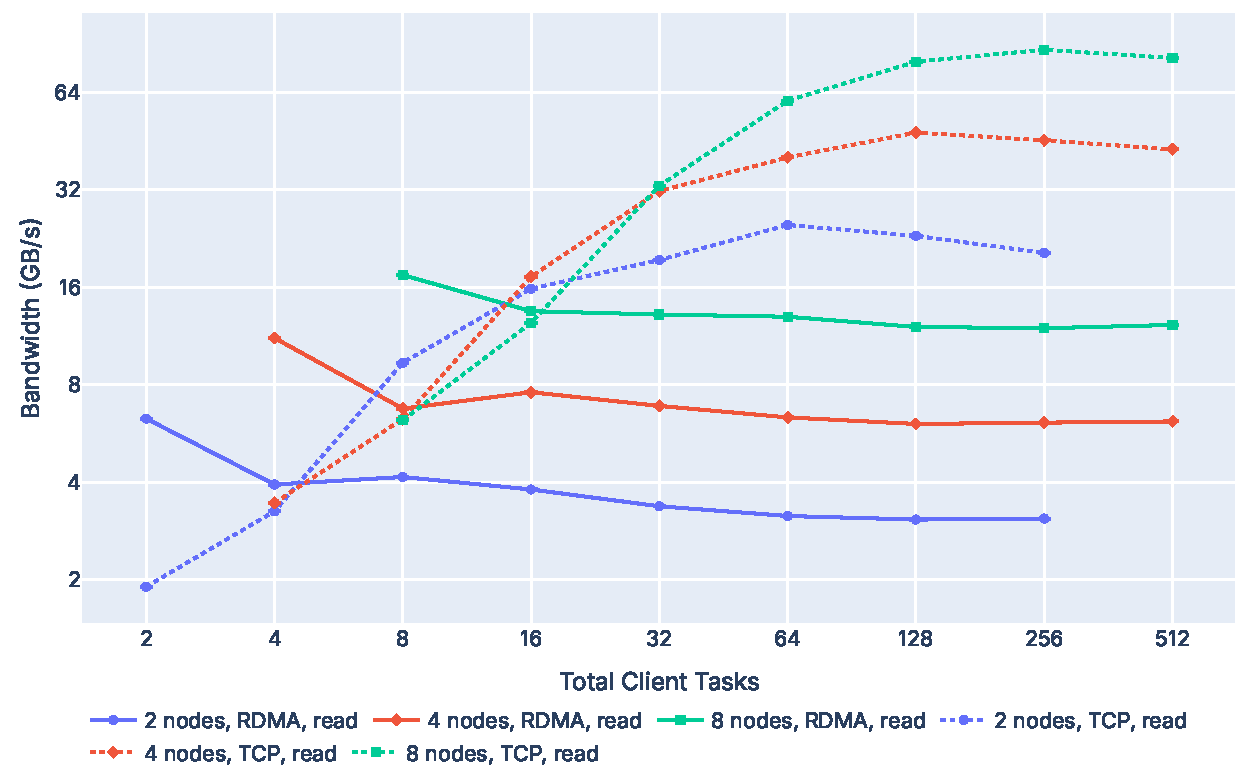
\includegraphics[width=0.9\linewidth]{assets/perf_results/rados_rdma_vs_tcp_seq_64m_read.pdf}
    \caption[RADOS RDMA/TCP Sequential Read Performance Comparison]{Comparison of 64MiB \acs{RADOS} reads using \acs{RDMA} and \acs{TCP} as the messenger backends.}
    \label{fig:rados-rdma-vs-tcp-seq-64m-read}
\end{figure}

\begin{figure}[H]
    \centering
    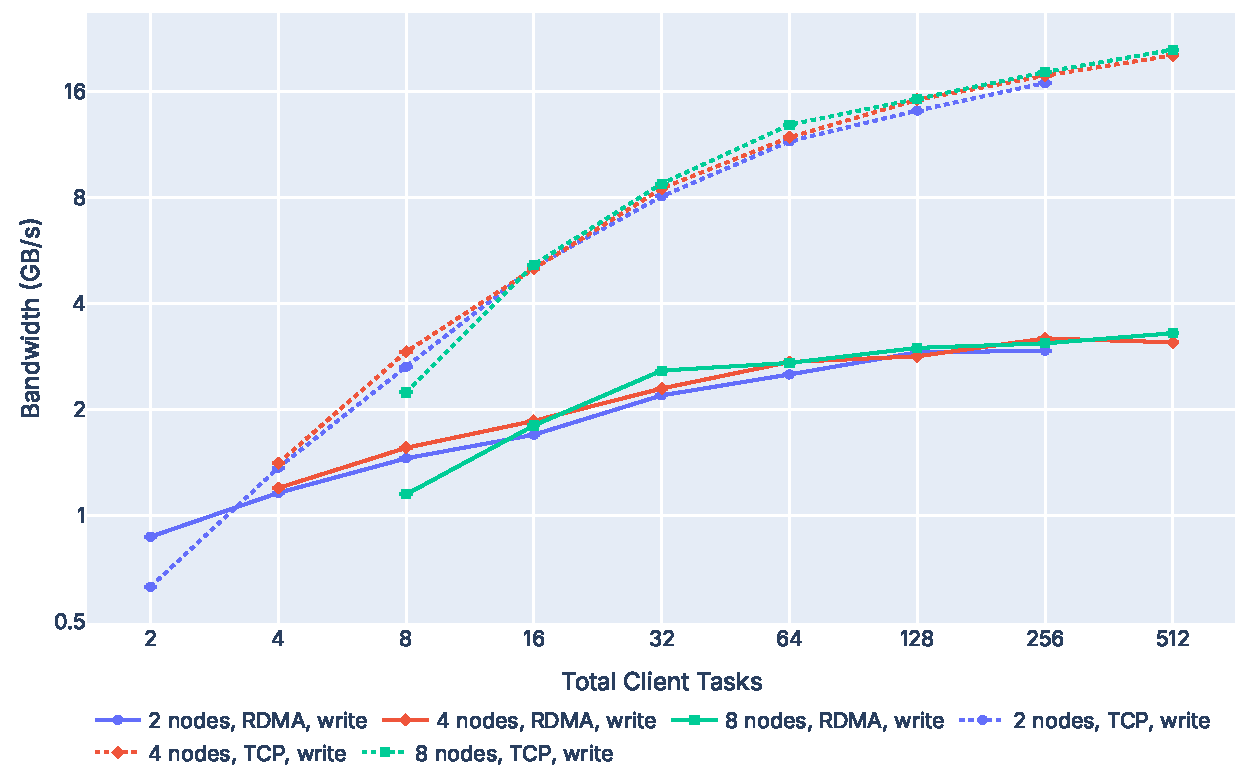
\includegraphics[width=0.9\linewidth]{assets/perf_results/rados_rdma_vs_tcp_seq_64m_write.pdf}
    \caption[RADOS RDMA/TCP Sequential Write Performance Comparison]{Comparison of 64MiB \acs{RADOS} writes using \acs{RDMA} and \acs{TCP} as the messenger backends.}
    \label{fig:rados-rdma-vs-tcp-seq-64m-write}
\end{figure}

\Cref{fig:rados-rdma-vs-tcp-seq-64m-read} demonstrates the unusual performance observed when using \ac{RDMA} as the messenger transport. Unlike \ac{TCP}, throughput scaling was not observed with increased task counts; performance immediately reached a per-node performance limitation. This resulted in performance at low numbers of tasks per node being $\approx3\times$ higher with \ac{RDMA} over \ac{TCP}, yet significantly lower at high task counts---\ac{TCP} performance was $\approx7\times$ higher than \ac{RDMA} at the maximum number of tasks per node.

\Cref{fig:rados-rdma-vs-tcp-seq-64m-write} additionally demonstrates poor write performance; regardless of the node count, write performance at the same number of tasks per node is nearly identical and generally significantly worse than that of \ac{TCP}, with the only exception being the performance at 2 total tasks. At the maximum task count, \ac{TCP} performance exceeded \ac{RDMA} performance by a factor of 6.5.

\subsubsection*{Small Object Operations}

\begin{figure}[H]
    \centering
    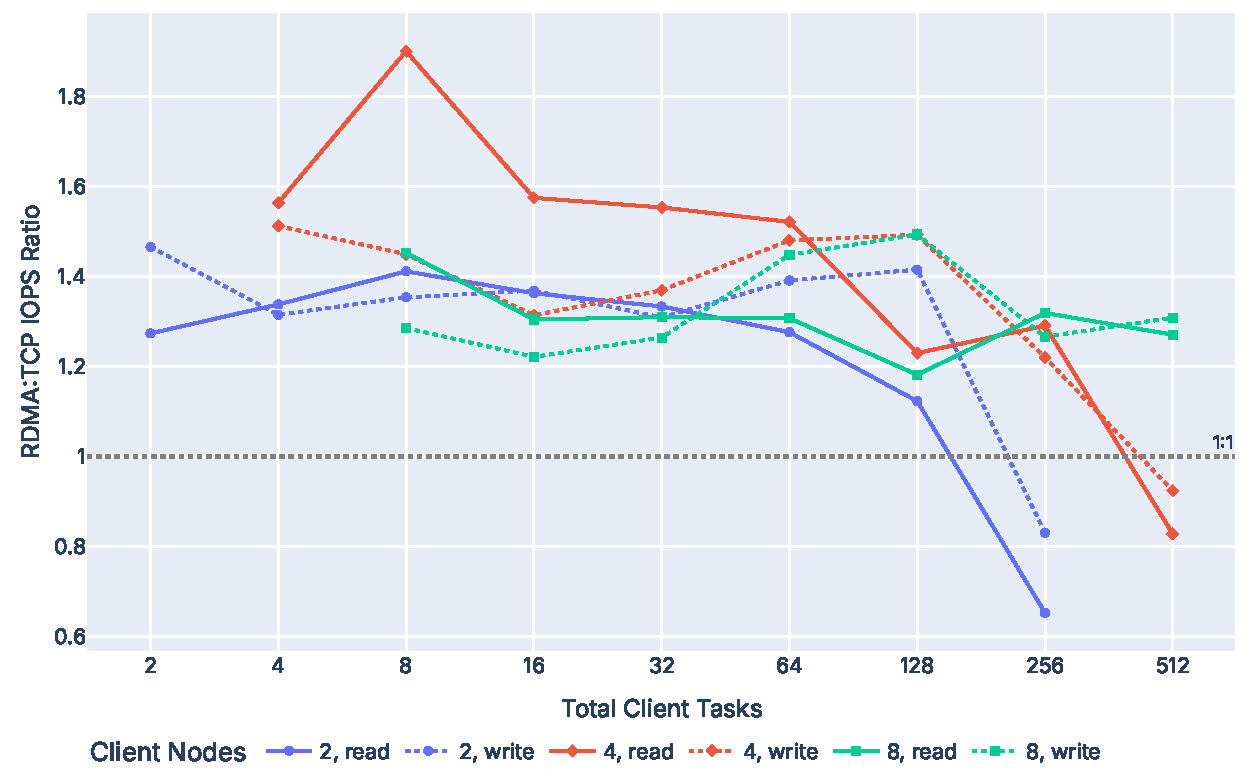
\includegraphics[width=0.9\linewidth]{assets/perf_results/rados_rdma_tcp_ratio_4k.pdf}
    \caption[RADOS RDMA/TCP 4KiB Write Performance Comparison]{Performance comparison between \acs{RDMA} and \acs{TCP} for 4KiB \ac{RADOS} operations.}
    \label{fig:rados-rdma-tcp-ratio-4k}
\end{figure}

\Cref{fig:rados-rdma-tcp-ratio-4k} shows that the performance of the \ac{RDMA} transport for small writes is modestly higher for most combinations of nodes and client tasks. In addition, although the performance at 2 nodes/256 tasks and 4 nodes/512 tasks is lower than that of the \ac{TCP} transport, the performance penalty is much less significant than for large read/write sizes; the lowest relative performance result shows \ac{TCP} outperforming \ac{RDMA} by a factor of 1.5, rather than the 6.5--7$\times$ observed in the large \ac{I/O} performance results.

\subsubsection{Additional Issues}

In addition to these performance issues, we also observed sporadic failures for the \ac{IOR} benchmark to complete at high task counts, with disconnection issues being shown only in Ceph logs, as shown in~\cref{lst:ceph-ib-full}. Due to stability issues with the \ac{RDMA} transport, we also could not perform additional \ac{CephFS} performance testing.

\lstinputlisting[
    language=ini,
    caption={Ceph InfiniBand Connection Dropout Messages},
    label={lst:ceph-ib-full},
    frame=single,
    breaklines=true,
    float
]{assets/ceph/infiniband_conn_drop.txt}

%%%%%%%%%%%%%%%%%%%%%%%%%%%%%%%%%%%%%%%%%%%%%%%%%%%%%%%%%%%%%%%%%%%%%%%%%%%%%%%%%%%%%%%%%%%%%%%%

\pagebreak
\subsection{Benchmark Configuration}

The system configuration for the benchmarks performed is shown in~\cref{tbl:benchmark-conditions}. Benchmarks where InfiniBand networking was used have the configuration as shown in~\cref{tbl:infiniband-system}, while Omni-Path nodes are configured as in~\cref{tbl:omnipath-system}. Due to the performance and stability issues observed in~\cref{sec:transport-comparison-rados}, \ac{TCP} was used for all of the following benchmarks.

\begin{table}[h]
\centering
\begin{tabular}{|ll|}
\hline
Ceph Nodes         & 7 \\
Client Nodes       & 2--8 \\
Colocation         & Separate server/client nodes \\
Client Tasks       & 2--512, $1\leq t \leq 128$ per node \\
Monitors           & 1 (on node 1) \\
Managers           & 1 (on node 1) \\
\acp{OSD}          & 48 (on nodes 2--7, 8 \acp{OSD}/node) \\
\ac{OSD} size      & 24 GiB/\ac{OSD} \\
\acp{MDS}          & 4 (on node 1) \\
Replicated Pool Type & Replica 3 \\
\multirow{2}{*}{Erasure-Coded Pool Type} & 4+2 (\acs{RADOS}/\acs{CephFS} data pool) \\
& Replica 3 (\acs{CephFS} metadata pool) \\
\hline
\end{tabular}
\caption{Benchmarking Conditions}
\label{tbl:benchmark-conditions}
\end{table}

\subsection{Large Sequential \acs{I/O} Operations}

In order to evaluate sequential \ac{I/O} performance, we used the \ac{IOR} benchmark with various configurations. The replicated configuration used a data pool with replica 3; for \ac{CephFS}, a secondary metadata pool with replica 3 was also created. The erasure coding configuration used 4 data chunks and 2 coding chunks for the data pool; however, the \ac{CephFS} metadata pool remains as replica 3, as replicated metadata pools are required for \ac{CephFS}.

\subsubsection{\acs{RADOS} -- Replicated}

For large \ac{I/O} operation tests, we used individual objects/files, each 64 MiB in size. Larger objects caused issues with the \ac{RADOS} backend due to its default size limit of 128 MiB. Adjusting the maximum object size is possible, however, this option is discouraged by Ceph for practicality reasons\footnote{\url{https://ceph.io/en/news/blog/2017/v12-1-4-luminous-rc-released/}. Accessed 23.02.2026.}.

\begin{figure}[H]
    \centering
    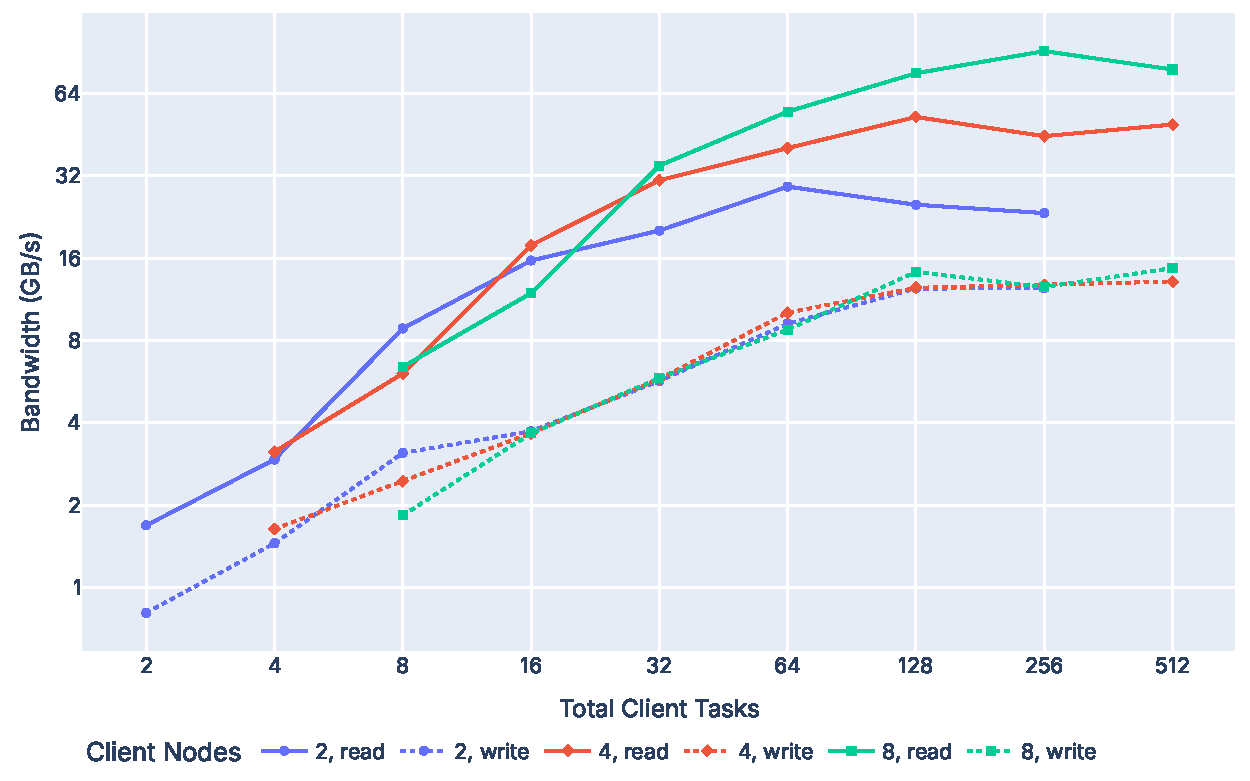
\includegraphics[width=\linewidth]{assets/perf_results/rados_tcp_seq_64m_repl3.pdf}
    \caption[RADOS 64MiB Sequential Read/Write I/O Performance]{Sequential read/write I/O performance using the \acs{RADOS} interface demonstrating scaling performance.}
    \label{fig:rados-tcp-seq-64m-repl3}
\end{figure}

\begin{figure}[H]
    \centering
    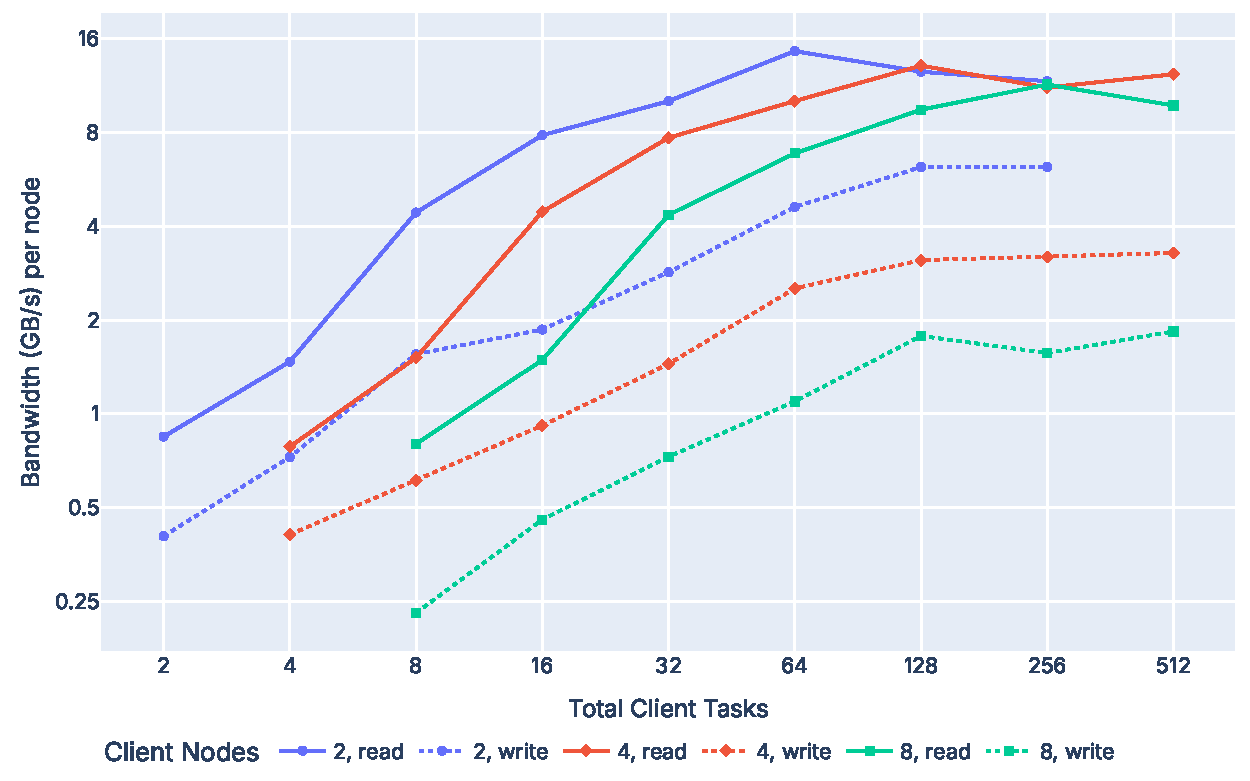
\includegraphics[width=\linewidth]{assets/perf_results/rados_tcp_seq_64m_repl3_pernode_normalized.pdf}
    \caption[RADOS 64MiB Sequential Read/Write I/O Performance (Normalized)]{Normalized sequential read I/O performance using the \acs{RADOS} interface showing per-node scaling limitations.}
    \label{fig:rados-tcp-seq-64m-repl3-pernode-normalized}
\end{figure}

\Cref{fig:rados-tcp-seq-64m-repl3} demonstrates the sequential \ac{I/O} performance with the \ac{RADOS} backend, showing strong scaling performance on reads limited primarily by per-node throughput. Normalizing the results as shown in \Cref{fig:rados-tcp-seq-64m-repl3-pernode-normalized} such that the Y-axis shows the total bandwidth per node, we can see near-linear scaling with the number of tasks per node up to a performance ceiling slightly over 100\ Gbit/s. This suggests that given a sufficient number of nodes, it is possible for Ceph to scale up further in terms of read performance. However, write performance is bottlenecked with an overall limit of 10--15 GB/s, regardless of the number of client nodes.

\begin{figure}[H]
    \centering
    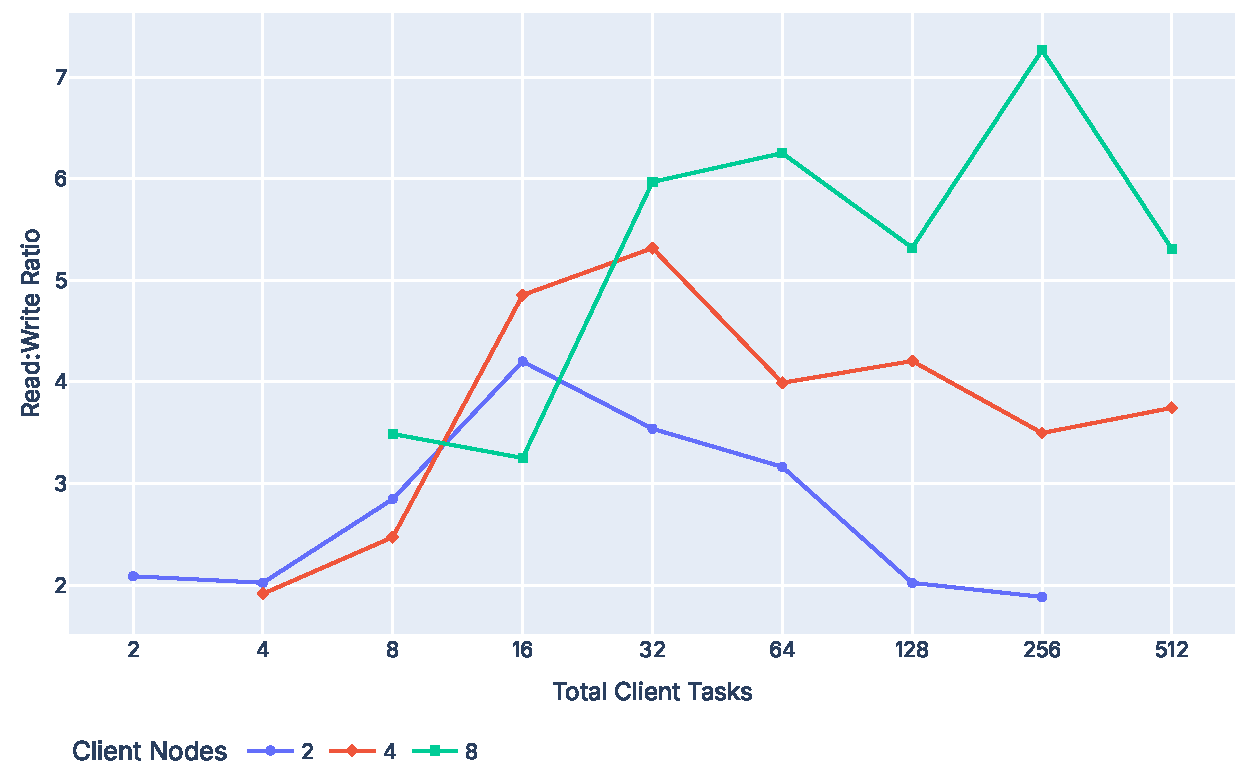
\includegraphics[width=\linewidth]{assets/perf_results/rados_tcp_seq_64m_repl3_wr_ratio.pdf}    
    \caption[RADOS 64MiB Sequential Read-Write Ratio]{\acs{I/O} performance ratio (read:write) demonstrating significant write overhead.}
    \label{fig:rados-tcp-seq-64m-repl3-wr-ratio}
\end{figure}

Write performance is limited to 10--15 GiB/s overall, regardless of the node count, which suggests a cluster-side limitation. Given that the cluster is set up in a replica-3 configuration, we expect that the read:write performance ratio would be approximately 3:1 in \acs{OSD}-performance-limited conditions. Due to the way in which Ceph performs replicated writes---the write is performed once by the client to the primary \ac{OSD}, which replicates it to the other \acp{OSD} in the group---network performance limitations are more likely to be a result of cluster-side bottlenecks. This is especially the case for our test cluster, as both the client and Ceph cluster nodes have identical hardware configurations. The actual read:write performance ratio, shown in~\cref{fig:rados-tcp-seq-64m-repl3-wr-ratio}, shows a much higher write performance penalty, especially at higher node counts when the system runs into the cluster-wide write performance bottlenecks. The read:write performance ratio does not fall below 2:1.

\subsubsection{\acs{RADOS} -- Erasure Coding}

\begin{figure}[H]
    \centering
    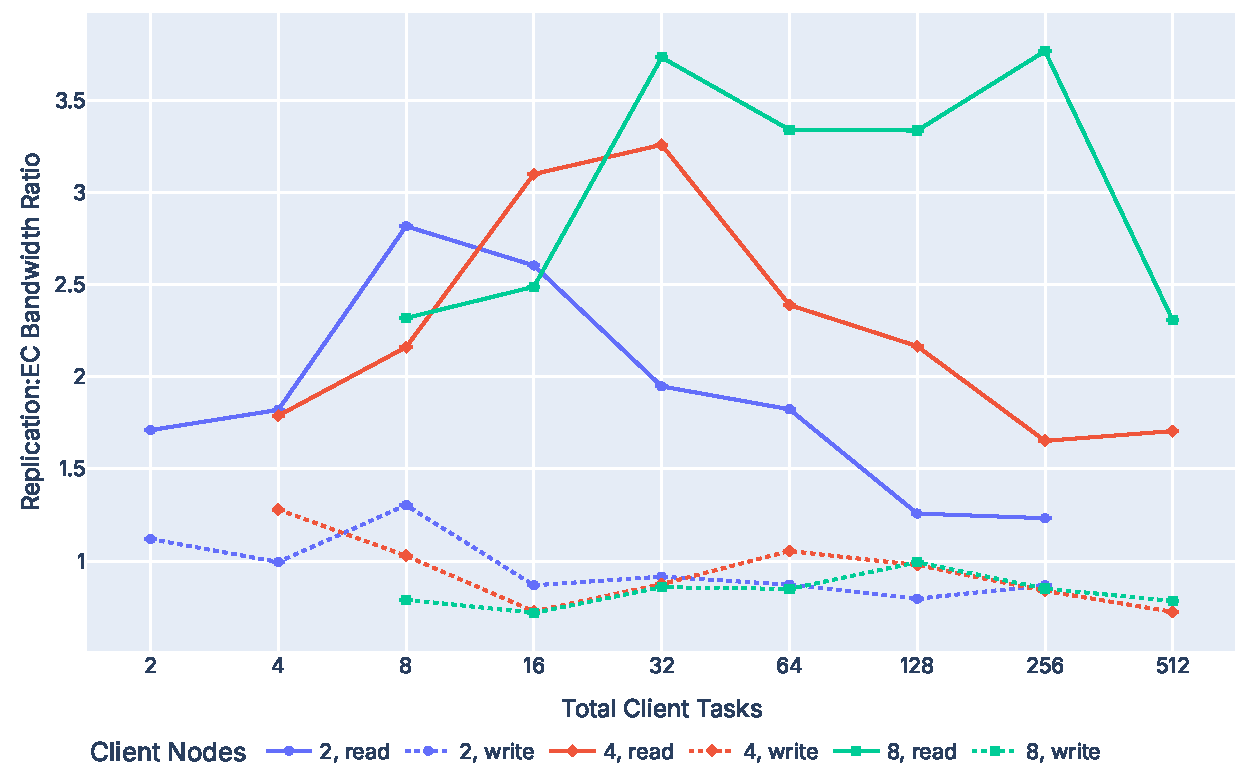
\includegraphics[width=\linewidth]{assets/perf_results/rados_tcp_repl_ec_ratio_seq_64m.pdf}
    \caption[\acs{RADOS} Erasure-Coding 64MiB Sequential Read/Write I/O Performance]{Sequential read/write \ac{I/O} performance of the \ac{RADOS} layer of replica-3 vs. 4+2 erasure-coding (EC) pools, demonstrating the performance impacts of erasure coding.}
    \label{fig:rados-tcp-repl-ec-ratio-seq-64m}
\end{figure}

\Cref{fig:rados-tcp-repl-ec-ratio-seq-64m} demonstrates the 4+2 erasure-coded read performance compared to replicated pools. In this configuration, a single object read results in the reading of data striped across all \acp{OSD}---since the \acp{OSD} are not bottlenecked by the underlying storage, \ac{EC} reads perform worse than standard replication. However, write performance behaviour with \ac{EC} is similar to that of replication, showing near-identical scaling. Overall, we observed that \ac{EC} writes at high client counts tended to perform better than replicated writes: this could be a result of the implicit striping performed by \ac{EC} across multiple \acp{OSD} reducing the overall write load on a single \ac{OSD}.

\pagebreak
\subsubsection{\acs{CephFS} -- Replicated}

\begin{figure}[H]
    \centering
    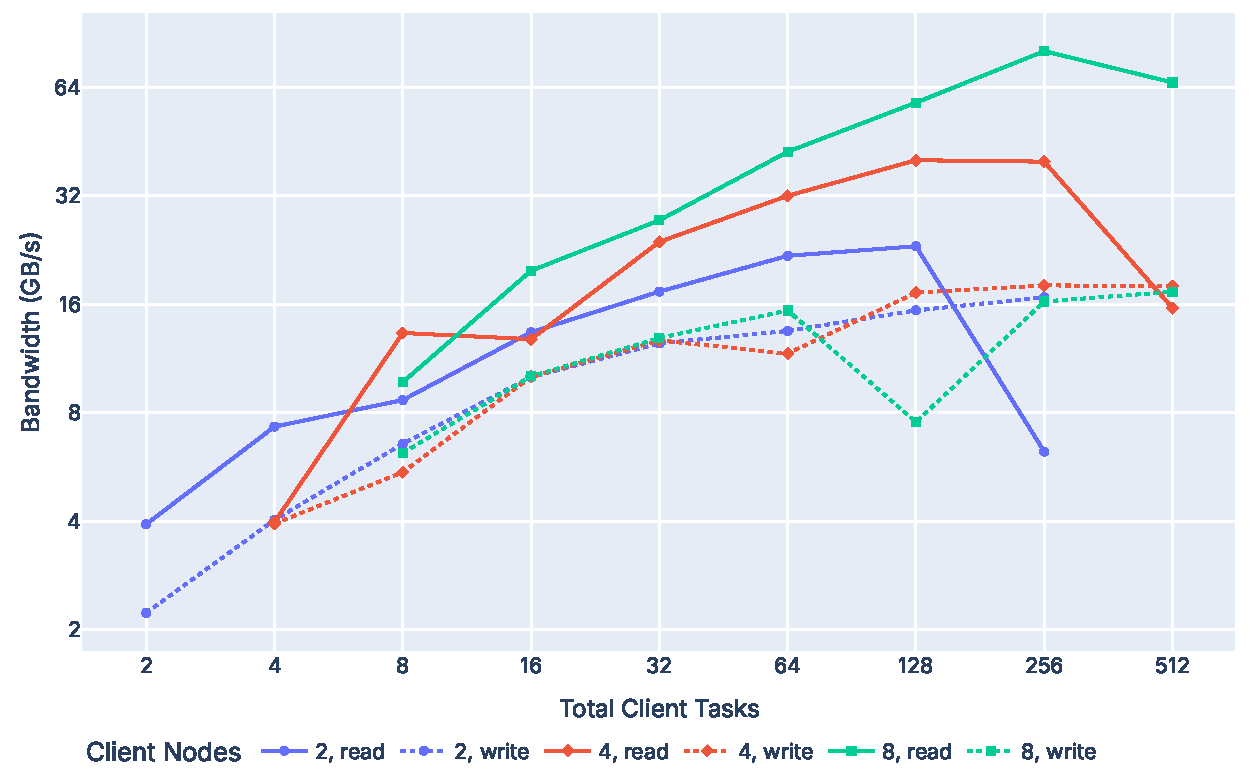
\includegraphics[width=0.9\linewidth]{assets/perf_results/cephfs_tcp_seq_64m_repl3.pdf}
    \caption[\acs{CephFS} 64MiB Sequential Read/Write I/O Performance]{Sequential read/write I/O performance using the \acs{CephFS} interface demonstrating scaling performance.}
    \label{fig:cephfs-tcp-seq-64m-repl3}
\end{figure}

\begin{figure}[H]
    \centering
    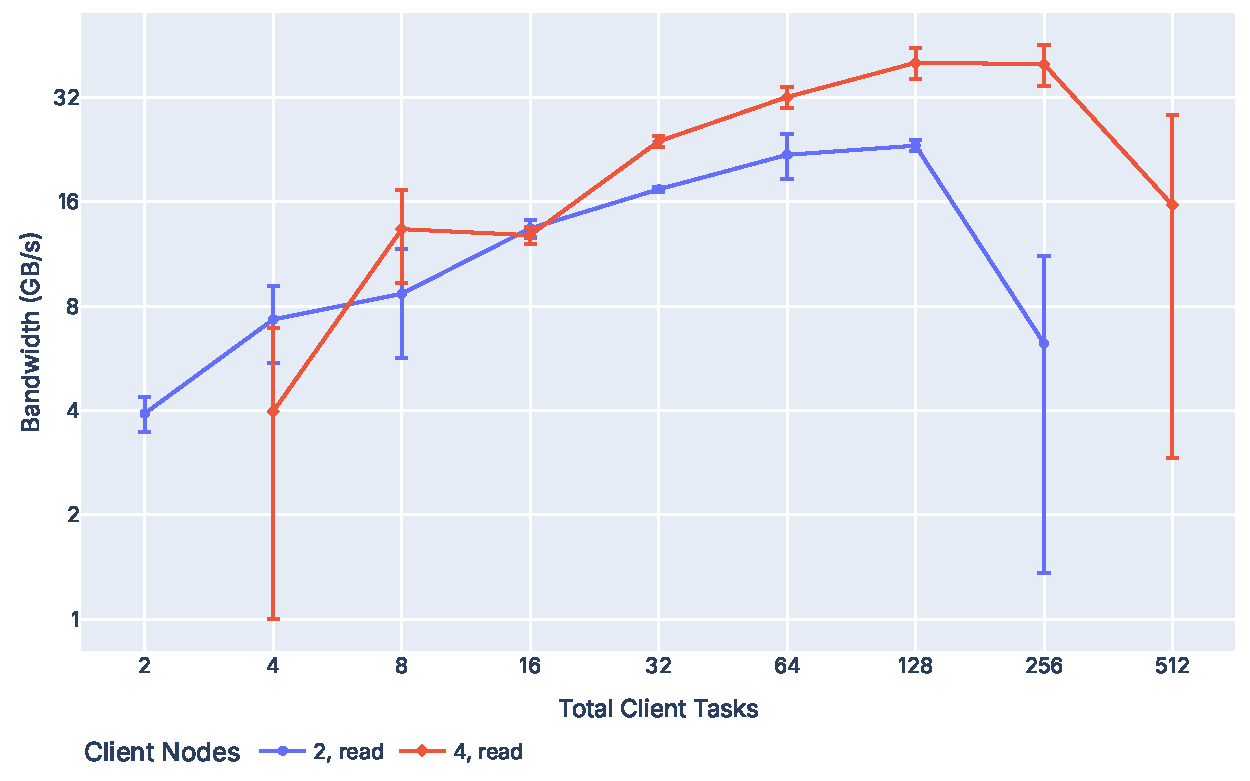
\includegraphics[width=0.9\linewidth]{assets/perf_results/cephfs_tcp_seq_64m_repl3_selected_error.pdf}
    \caption[\acs{CephFS} 64MiB Sequential Read/Write I/O Performance Variance]{Selected read performance plots of the \acs{CephFS} backend, showing unstable performance.}
    \label{fig:cephfs-tcp-seq-64m-repl3-selected-error}
\end{figure}

\Cref{fig:cephfs-tcp-seq-64m-repl3} shows similar sequential \ac{I/O} performance and scaling behaviour to that of the \ac{RADOS} backend, with the exception of an increased number of outliers, such as the performance drop in read performance for the tests involving 2 nodes/256 tasks and 4 nodes/512 tasks. Isolating these traces in~\cref{fig:cephfs-tcp-seq-64m-repl3-selected-error} shows very high performance variations for the outliers. Given that both of these tasks are using all available cores on the client nodes, this could be a result of \ac{CPU} time contention on the client side rather than performance bottlenecks on the cluster side. It is possible that the \ac{CephFS} layer, being more complex, is more \ac{CPU}-intensive than the \ac{RADOS} layer, leading to \ac{CPU} contention.

\subsubsection{\acs{CephFS} -- Erasure Coding}

\begin{figure}[H]
    \centering
    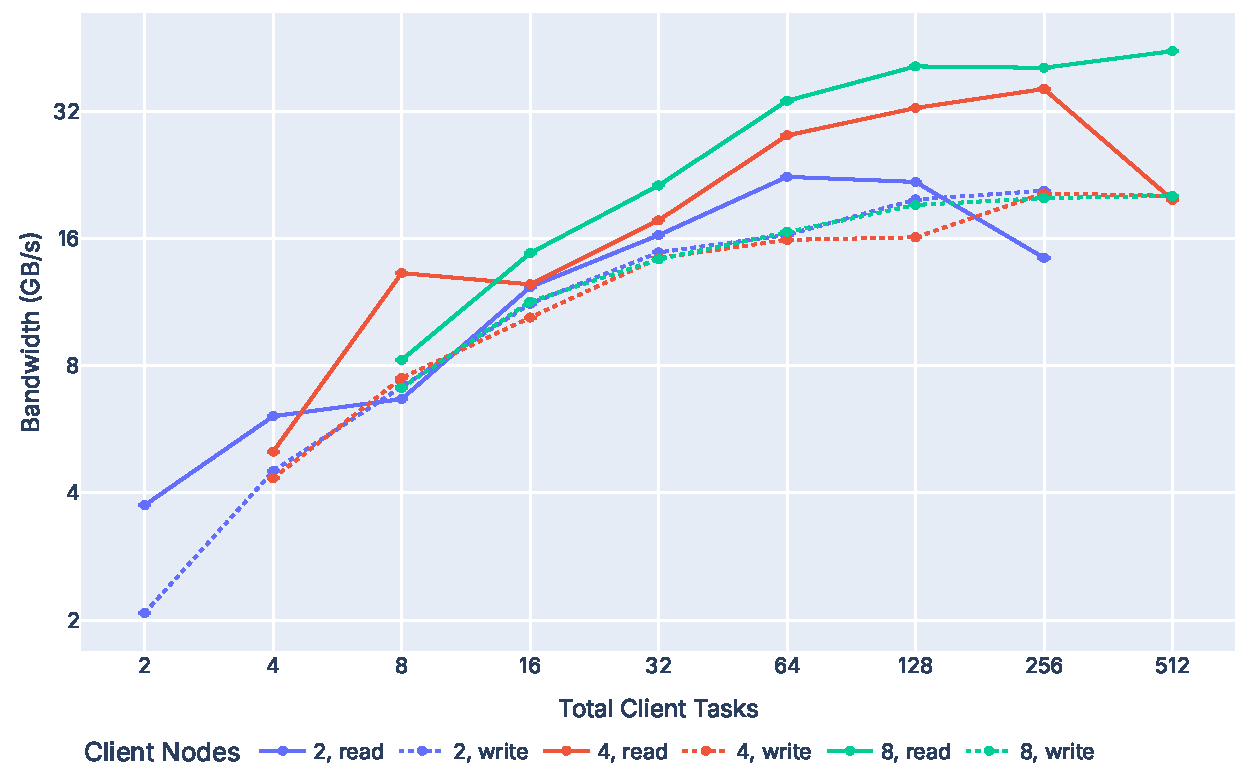
\includegraphics[width=0.9\linewidth]{assets/perf_results/cephfs_ec_seq_64m.pdf}
    \caption[\acs{CephFS} Erasure-Coding 64MiB Sequential Read/Write I/O Performance]{Sequential read/write \acs{I/O} performance of the \acs{CephFS} backend on a mixed 4+2 EC data and replica-3 metadata pool.}
    \label{fig:cephfs-ec-seq-64m}
\end{figure}

\Cref{fig:cephfs-ec-seq-64m} shows similar scaling to that of the replicated configuration. The dropoff in performance for the 2-node/256-task and 4-node/512-task remains, but to a lesser extent than the replicated configuration. Overall performance is more complex: \Cref{fig:cephfs-tcp-ec-ratio-seq-64m} demonstrates that, unlike \ac{RADOS}, the overhead of \ac{EC} is less significant: read performance was somewhat slower than the replicated performance, while write performance with \ac{EC} was generally identical to, or better than, replication. We also observed consistently that in the suspected \acs{CPU}-bottlenecked scenario with 2-node/256-task and 4-node/512-task runs, performance was significantly higher than that of the replicated runs.

\begin{figure}[H]
    \centering
    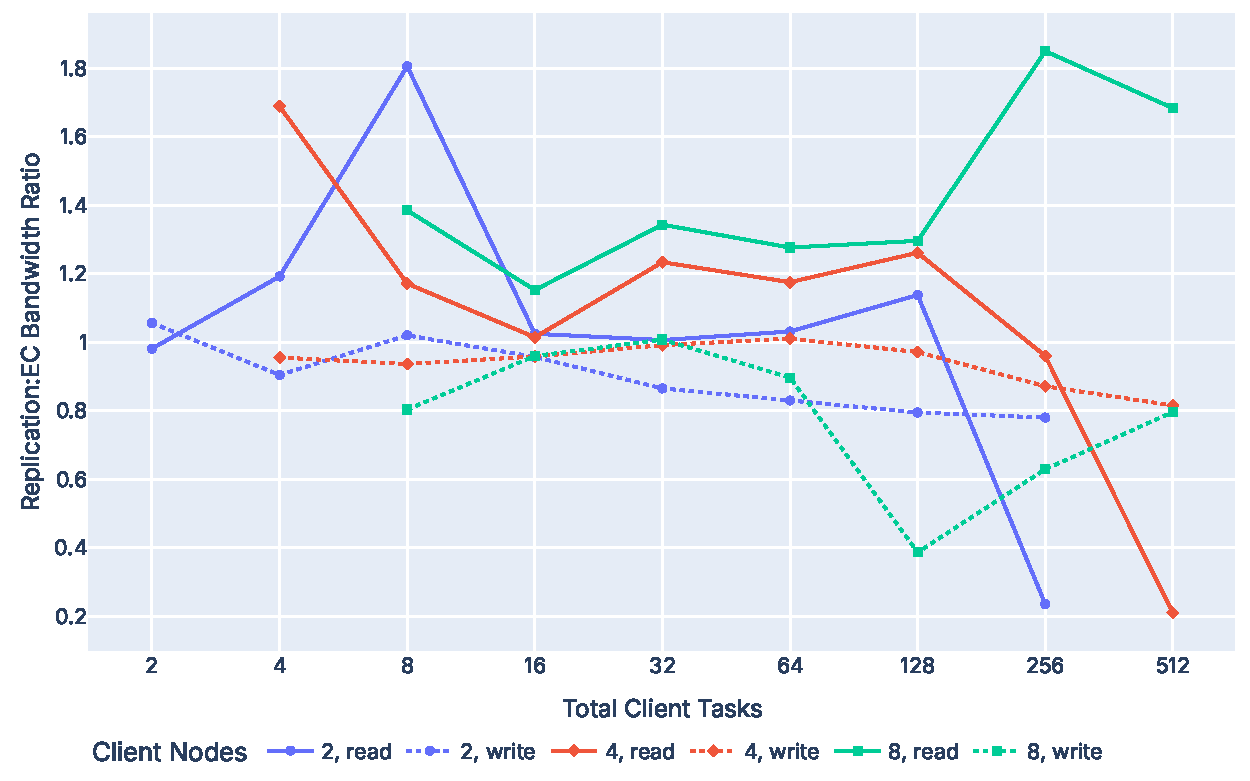
\includegraphics[width=0.9\linewidth]{assets/perf_results/cephfs_tcp_repl_ec_ratio_seq_64m.pdf}
    \caption[\acs{CephFS} Erasure-Coding 64MiB Sequential Read/Write Performance Ratio]{Relative performance ratio of replication over \acs{EC} for the \acs{CephFS} backend.}
    \label{fig:cephfs-tcp-ec-ratio-seq-64m}
\end{figure}

\subsection{Small \acs{I/O} Operations}

For small \ac{I/O} tests on the \ac{RADOS} layer, 2MiB objects were created and written to in 4 KiB increments. For the \ac{CephFS} layer, we additionally performed tests with and without fsync enabled. The behaviour of the \ac{RADOS} backend within \ac{IOR} is not affected by fsync options, as \ac{IOR} uses the synchronous operations provided by the \ac{RADOS} \ac{API}.

\subsubsection{Replicated Performance}

\begin{figure}[htbp]
    \centering
    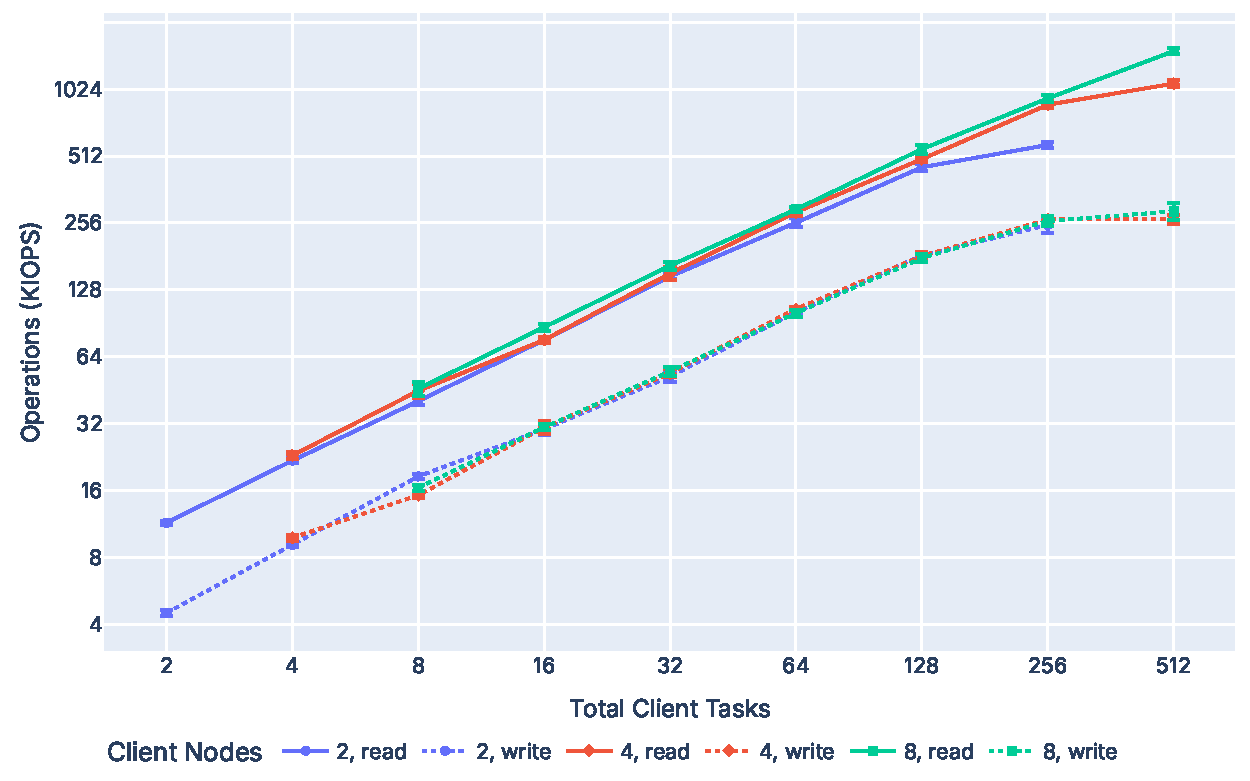
\includegraphics[width=0.9\linewidth]{assets/perf_results/rados_tcp_seq_4k_2m_repl3.pdf}
    \caption[RADOS 4KiB Sequential Read/Write I/O Performance]{Sequential 4KiB read/write I/O performance using the \acs{RADOS} interface.}
    \label{fig:rados-tcp-seq-4k-2m-repl3}
\end{figure}

\Cref{fig:rados-tcp-seq-4k-2m-repl3} shows per-client performance limitations with the \ac{RADOS} backend; read performance is limited to $\leq$ 6K \ac{IOPS} per task, while write performance is limited to $\leq$ 2.5K \ac{IOPS} per task. Unlike the large sequential write results, the performance drop-off at high task counts is much smaller; per-node limitations are also less apparent for small \ac{I/O} operations, likely due to the impacts of network latency. Variance in \ac{IOPS} between runs is low.

\begin{figure}[htbp]
    \centering
    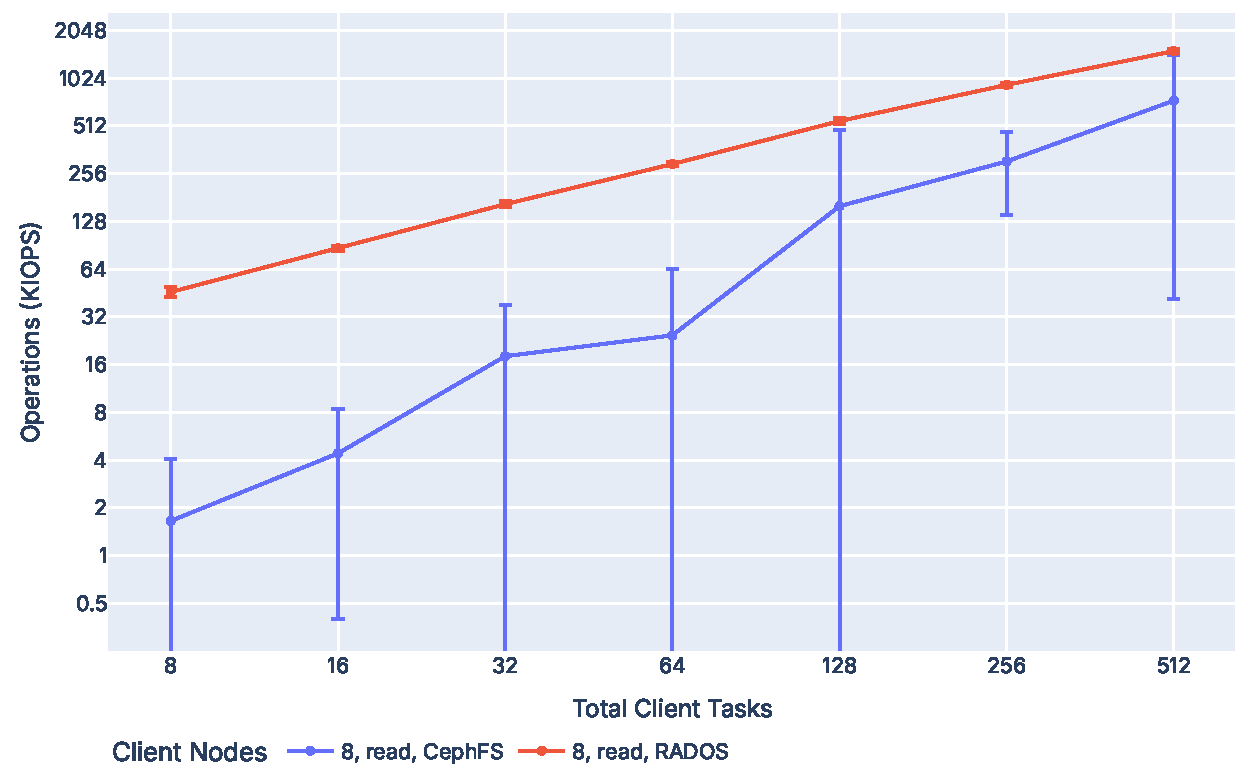
\includegraphics[width=0.9\linewidth]{assets/perf_results/cephfs_tcp_seq_4k_2m_8N.pdf}
    \caption[\acs{CephFS} 4KiB Sequential Read I/O Performance]{Sequential 4KiB read I/O performance for 8 nodes using the \acs{CephFS} interface compared to the \acs{RADOS} interface showing high performance variance.}
    \label{fig:cephfs-tcp-seq-4k-2m-repl3-8N}
\end{figure}

Unlike \ac{RADOS}, \ac{CephFS} demonstrates much higher performance variation. In~\cref{fig:cephfs-tcp-seq-4k-2m-repl3-8N}, we have selected only the 8-node results for readability purposes; however, for all tests, performance is both significantly lower than that of \ac{RADOS}, and variance is significantly higher. This is especially apparent at low client node counts: at 8 nodes and 1 task/node, 4KB sequential reads are 27$\times$ higher on the \ac{RADOS} backend (45.9K \acs{IOPS}) compared to \ac{CephFS} (1.65K \acs{IOPS}). 

\begin{figure}[htbp]
    \centering
    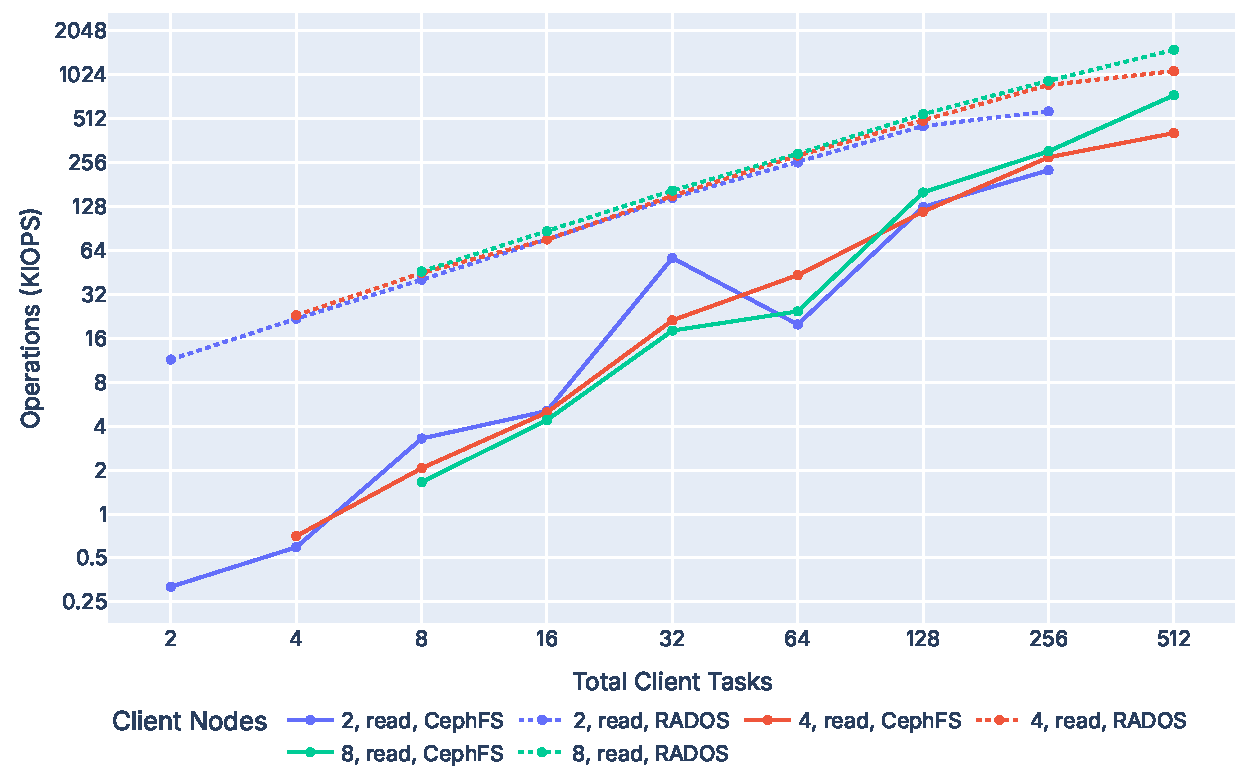
\includegraphics[width=0.9\linewidth]{assets/perf_results/cephfs_tcp_seq_4k_2m_8N_rd_comparison.pdf}
    \caption[\acs{CephFS}/\acs{RADOS} 4KiB Sequential Read I/O Comparison]{Comparison of 4KiB sequential read performance between the \acs{RADOS} and \acs{CephFS} backends, showing similar scaling despite significantly lower performance with \acs{CephFS}.}
    \label{fig:cephfs-tcp-seq-4k-2m-repl3-8N-rd}
\end{figure}

However, although the variance is higher with lower performance, the scaling behaviour is similar to that of the \ac{RADOS} backend as the node count is increased, as shown in~\cref{fig:cephfs-tcp-seq-4k-2m-repl3-8N-rd}.

\begin{figure}[htbp]
    \centering
    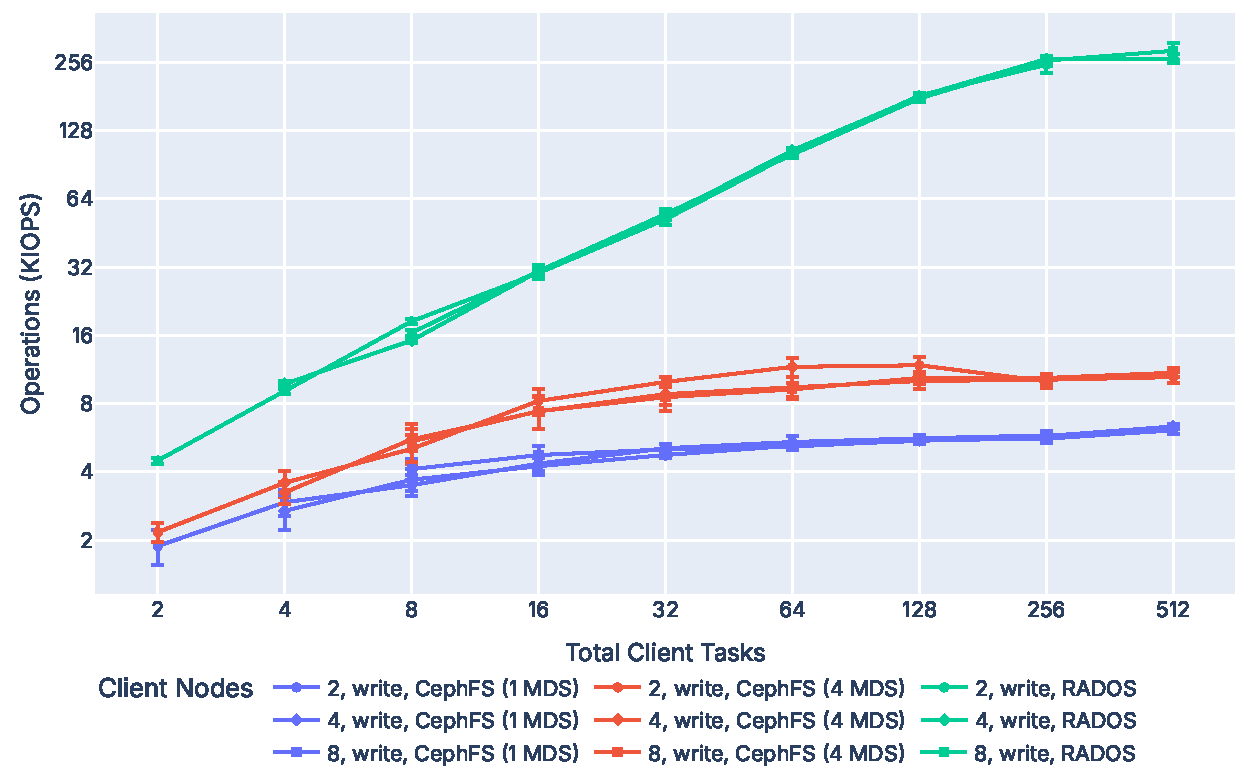
\includegraphics[width=0.9\linewidth]{assets/perf_results/cephfs_tcp_seq_4k_2m_write.pdf}
    \caption[\acs{CephFS}/\acs{RADOS} 4KiB Sequential Write I/O Comparison]{Comparison of 4KiB sequential write performance between the \acs{RADOS} and \acs{CephFS} backends.}
    \label{fig:cephfs-tcp-seq-4k-2m-repl3-8N-wr}
\end{figure}

Write performance on \ac{CephFS}, as shown in~\cref{fig:cephfs-tcp-seq-4k-2m-repl3-8N-wr} is more consistent compared to read performance. However, the \ac{IOPS} seem to be limited by the performance of the \ac{MDS}: a single \ac{MDS} produced approximately 6 k\acs{IOPS} of write performance, while 4 \ac{MDS} daemons with distributed ephemeral pinning enabled produced up to 11 k\acs{IOPS}. The increased number of \ac{MDS} daemons only increased performance if both distributed ephemeral pinning was enabled on the benchmarking folder and when each task created a unique directory; otherwise, performance results for the single \ac{MDS} and 4-\ac{MDS} configuration were identical. The overhead compared to \ac{RADOS} is additionally lower for writes.

\subsubsection{\acs{CephFS} -- Erasure Coding}

\begin{figure}[htbp]
    \centering
    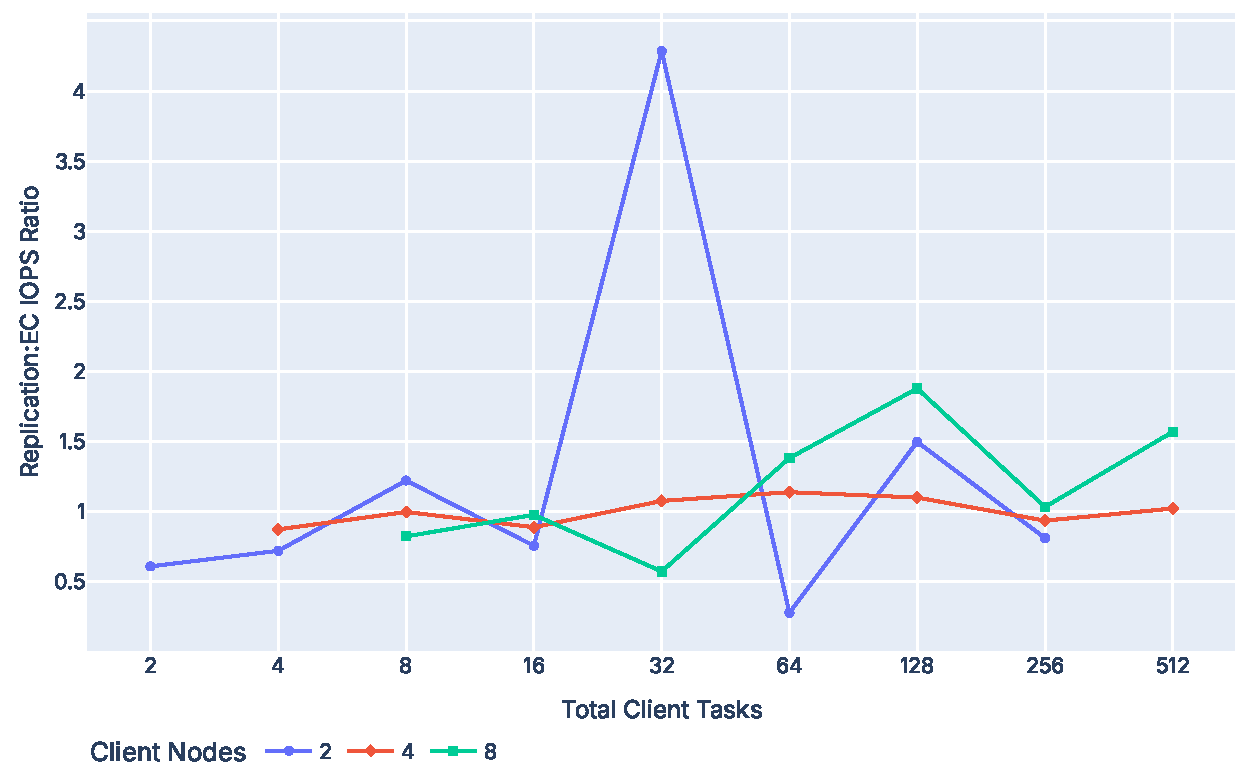
\includegraphics[width=0.9\linewidth]{assets/perf_results/cephfs_repl_ec_ratio_4k_read.pdf}
    \caption[\acs{CephFS} 4KiB Sequential Read I/O Comparison]{Relative read performance of erasure coding over replicated pools with the \acs{CephFS} backend. A higher ratio represents higher replicated performance relative to erasure coding.}
    \label{fig:cephfs-repl-ec-ratio-4k-read}
\end{figure}

\begin{figure}[htbp]
    \centering
    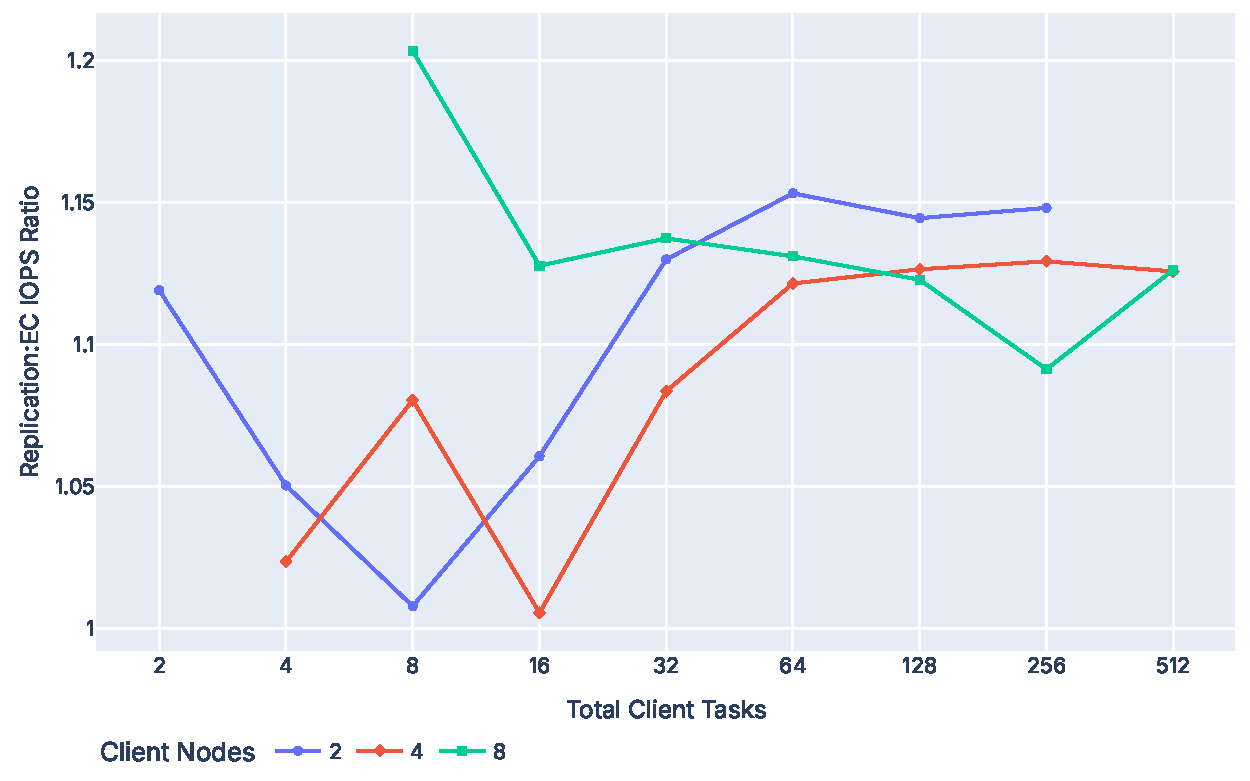
\includegraphics[width=0.9\linewidth]{assets/perf_results/cephfs_repl_ec_ratio_4k_write.pdf}
    \caption[\acs{CephFS} 4KiB Sequential Write I/O Comparison]{Relative write performance of erasure coding over replicated pools with the \acs{CephFS} backend. A higher ratio represents higher replicated performance relative to erasure coding.}
    \label{fig:cephfs-repl-ec-ratio-4k-write}
\end{figure}

\Cref{fig:cephfs-repl-ec-ratio-4k-read}~and~\cref{fig:cephfs-repl-ec-ratio-4k-write} demonstrate the read and write performance ratio of replicated pools over erasure coded \acs{CephFS} pools. Except for an outlier at 2 nodes/32 tasks and 2 nodes/64 tasks, small erasure-coded writes of relatively large objects (2MiB) are not consistently faster or slower than that of replicated writes. Write performance with \ac{CephFS} shows a minor performance penalty for erasure-coding up to approximately 20\% relative to replication, which was observed at 8 nodes/8 tasks.
